% =====================================================================
%  W3C PROV / PROV-Agent meta-model (the abstract base ontology)
% ---------------------------------------------------------------------
%  Standalone TikZ figure. Compile with any modern TeX Live:
%
%      pdflatex prov-metamodel-ontology.tex
%      latexmk -pdf prov-metamodel-ontology.tex     % cropped PDF
%
%  Required packages (all ship with a standard TeX Live / MiKTeX):
%      standalone, tikz (+ libraries below), xcolor
%
%  Visual notation follows W3C PROV, with the conventional PROV class
%  colours (muted for print):
%      Entity   = ellipse   (soft yellow)
%      Activity = rectangle (soft blue)
%      Agent    = pentagon  (soft orange)
%
%  This is the generic model that Layer 2 (omd-provagent-ontology.tex)
%  instantiates and extends with domain relations. PROV-Agent adds the
%  agent-centric associations for agentic AI workflows (arXiv:2508.02866).
%
%  Recommended paper caption: see prov-metamodel-caption.md
% =====================================================================
\documentclass[border=10pt]{standalone}

\usepackage{xcolor}
\usepackage{tikz}
\usetikzlibrary{arrows.meta, positioning, shapes.geometric, calc}

% --- palette: muted grayscale base + conventional PROV class colours ---
\definecolor{ink}{HTML}{1A1A1A}
\definecolor{edge}{HTML}{404040}
\definecolor{muted}{HTML}{6B6B6B}
\definecolor{entfill}{HTML}{FBF3D3}   % PROV entity   — soft yellow
\definecolor{entline}{HTML}{9C8B33}
\definecolor{actfill}{HTML}{DDE7F7}   % PROV activity — soft blue
\definecolor{actline}{HTML}{3F6FB0}
\definecolor{agtfill}{HTML}{FBE1C0}   % PROV agent    — soft orange
\definecolor{agtline}{HTML}{BE843A}

% --- output size: ONE knob. Rescales the whole figure (shapes + text)
%     uniformly. Default 0.7 emits a compact PDF; set 1.0 for full size.
%     In the paper you can instead size it at include time, e.g.
%       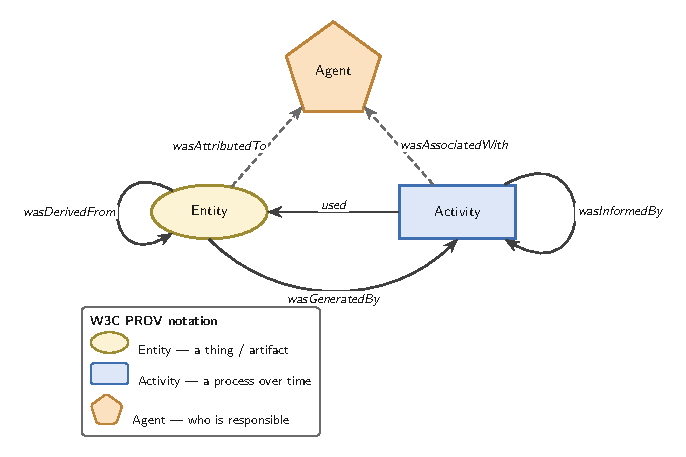
\includegraphics[width=0.7\textwidth]{prov-metamodel-ontology}
\newcommand{\figscale}{0.7}

\begin{document}
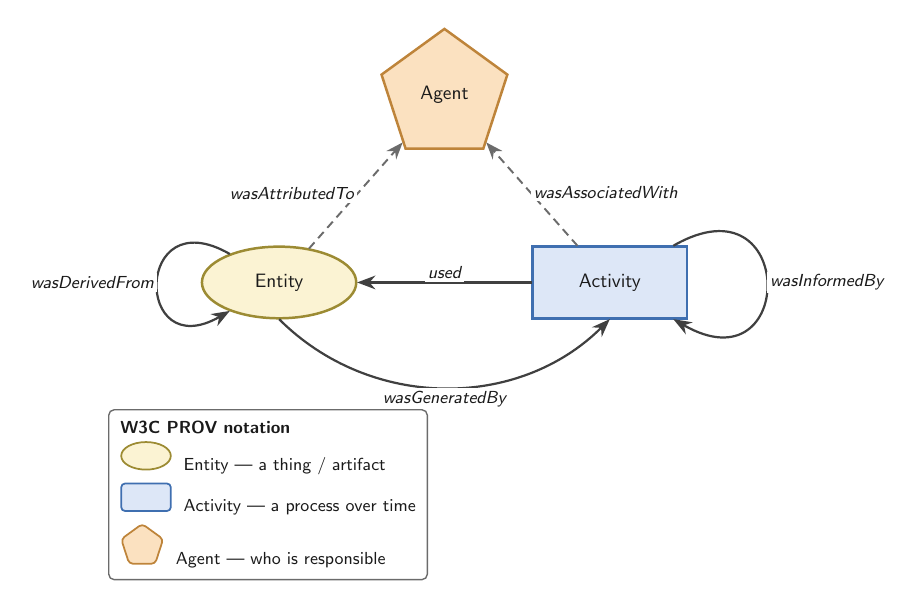
\begin{tikzpicture}[
    scale=\figscale, transform shape,
    font=\sffamily,
    >=Stealth,
    entity/.style={
        ellipse, draw=entline, line width=0.9pt, fill=entfill,
        text=ink, align=center, inner sep=2pt, font=\sffamily,
        minimum width=28mm, minimum height=13mm},
    activity/.style={
        rectangle, draw=actline, line width=0.9pt, fill=actfill,
        text=ink, align=center, inner sep=3pt, font=\sffamily,
        minimum width=28mm, minimum height=13mm},
    agent/.style={
        regular polygon, regular polygon sides=5, draw=agtline,
        line width=0.9pt, fill=agtfill, text=ink, inner sep=1pt,
        font=\sffamily, minimum width=24mm},
    rel/.style={->, line width=0.8pt, draw=edge},
    aedge/.style={->, line width=0.7pt, draw=muted, densely dashed},
    lab/.style={font=\sffamily\small\itshape, text=ink,
                fill=white, inner sep=1.6pt},
]

% --- the three PROV classes ------------------------------------------
\node[entity]   (E) at (0,0)   {Entity};
\node[activity] (A) at (6,0)   {Activity};
\node[agent]    (G) at (3,3.4) {Agent};

% --- the six core relations ------------------------------------------
% used: activity used an entity
\draw[rel] (A) -- node[lab,above]{used} (E);
% wasGeneratedBy: entity generated by activity (arc below)
\draw[rel] (E.south) to[out=-45,in=-135]
           node[lab,below]{wasGeneratedBy} (A.south);
% wasDerivedFrom: entity from entity (self-loop, left)
\draw[rel] (E) to[out=150,in=210,looseness=5]
           node[lab,left]{wasDerivedFrom} (E);
% wasInformedBy: activity from activity (self-loop, right)
\draw[rel] (A) to[out=30,in=-30,looseness=5]
           node[lab,right]{wasInformedBy} (A);
% agent associations (dashed)
\draw[aedge] (A) -- node[lab,pos=0.52,right]{wasAssociatedWith} (G);
\draw[aedge] (E) -- node[lab,pos=0.52,left]{wasAttributedTo} (G);

% --- shape key (compact, lower strip) --------------------------------
\node[anchor=north west, align=left, font=\sffamily\small, text=ink,
      draw=muted, line width=0.5pt, rounded corners=2pt, inner sep=6pt]
      at (-3.1,-2.3)
{\textbf{W3C PROV notation}\\[3pt]
 \tikz\node[entity,minimum width=9mm,minimum height=5mm,inner sep=0pt]{};\ \ Entity — a thing / artifact\\[3pt]
 \tikz\node[activity,minimum width=9mm,minimum height=5mm,inner sep=0pt]{};\ \ Activity — a process over time\\[3pt]
 \tikz\node[agent,minimum width=8mm,inner sep=0pt]{};\ \ Agent — who is responsible};

\end{tikzpicture}
\end{document}
